\documentclass[10pt,a4paper]{article}

%double si on veut une version prof et une version élève. simple si on veut une seule version.
\newcommand{\buildmode}{simple}

\InputIfFileExists{version.tex}{}{}
% Version (définie par le script)
\providecommand{\version}{eleve}

\usepackage{feuilleinterro}

%%%à modifier à chaque fois

\renewcommand{\niveau}{1STMG}
\renewcommand{\chapitre}{Fonctions, généralités}
\renewcommand{\numchap}{0.1}
\renewcommand{\theme}{Fonctions}

\begin{document}

% =========================================================
% PAGE 1 : VERSIONS A ET B
% =========================================================

\begin{sujets}

\interroversion{A}

\textbf{Exercice 1 -- Tableau de valeurs \hfill /2}

On considère la fonction \(f\) définie sur \(\mathbb{R}\) par \(f(x)=x^2-2x-3\).

Complétez le tableau de valeurs suivant (une valeur est déjà calculée à titre d'exemple : \(f(1)=1^2-2\times 1-3=-4\)).

\begin{center}
    \renewcommand{\arraystretch}{1.5}
    \setlength{\tabcolsep}{0.25cm}
    \begin{tabular}{|*{7}{c|}}
    \hline
    \(x\) & \(-2\) & \(-1\) & \(0\) & \(1\) & \(2\) & \(3\) \\
    \hline
    \(f(x)\) & & \(0\) & & \(-4\) & \(-3\) & \(0\) \\
    \hline
    \end{tabular}
\end{center}

\vspace{3cm}

\textbf{Exercice 2 -- Lecture graphique \hfill /3}

On considère une fonction \(h\) dont la représentation graphique est donnée ci-dessous.

\begin{center}
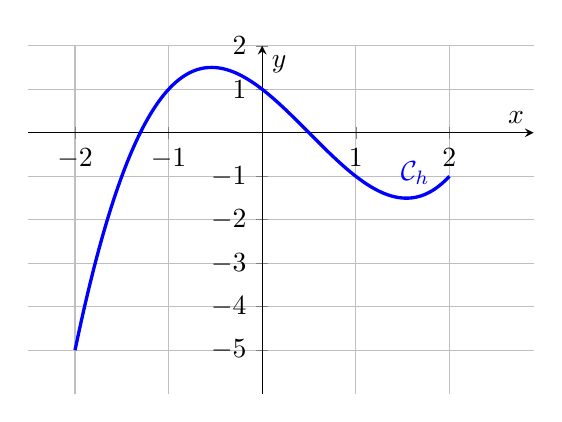
\begin{tikzpicture}
\begin{axis}[
    axis lines=middle,
    xmin=-2.5, xmax=2.9,
    ymin=-6, ymax=2,
    domain=-2:2,
    samples=300,
    grid=major,
    xtick={-2,-1,0,1,2,3},
    ytick={-5,-4,-3,-2,-1,0,1,2,3,4},
    xlabel={\(x\)},
    ylabel={\(y\)},
    width=8cm,
    height=6cm
]
\addplot[blue, very thick] {2/3*(x-2)*(x+1.5)*(x-1)-1}
node[pos=0.92, above right] {\(\mathcal{C}_h\)};
\end{axis}
\end{tikzpicture}
\end{center}

\begin{enumerate}
    \item Quel est l'ensemble de définition de \(h\) ? \hfill /1
    \item Donner les images de \(-2\), \(0\) et \(1\) par \(h\). \hfill /1
    \item Donner les éventuels antécédents de \(-1\) et de \(1\). \hfill /1
\end{enumerate}

\columnbreak

\interroversion{B}

\textbf{Exercice 1 -- Tableau de valeurs \hfill /2}

On considère la fonction \(f\) définie sur \(\mathbb{R}\) par \(f(x)=x^2+x-2\).

Complétez le tableau de valeurs suivant (une valeur est déjà calculée à titre d'exemple : \(f(2)=2^2+2-2=4\)).

\begin{center}
    \renewcommand{\arraystretch}{1.5}
    \setlength{\tabcolsep}{0.25cm}
    \begin{tabular}{|*{7}{c|}}
    \hline
    \(x\) & \(-2\) & \(-1\) & \(0\) & \(1\) & \(2\) & \(3\) \\
    \hline
    \(f(x)\) & \(0\) & & \(-2\) & \(0\) & \(4\) & \\
    \hline
    \end{tabular}
\end{center}

\vspace{3cm}

\textbf{Exercice 2 -- Lecture graphique \hfill /3}

On considère une fonction \(h\) dont la représentation graphique est donnée ci-dessous.

\begin{center}
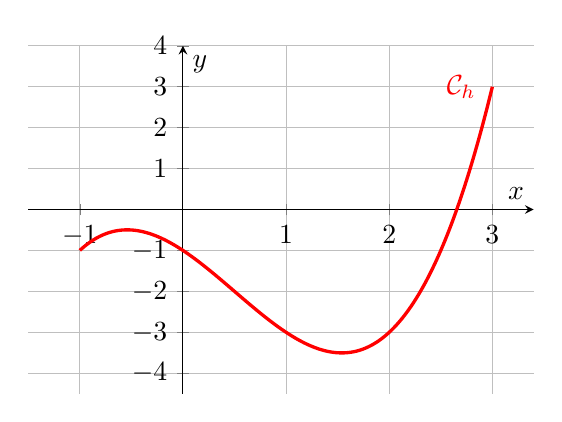
\begin{tikzpicture}
\begin{axis}[
    axis lines=middle,
    xmin=-1.5, xmax=3.4,
    ymin=-4.5, ymax=4,
    domain=-1:3,
    samples=300,
    grid=major,
    xtick={-2,-1,0,1,2,3,4},
    ytick={-4,-3,-2,-1,0,1,2,3,4},
    xlabel={\(x\)},
    ylabel={\(y\)},
    width=8cm,
    height=6cm
]
\addplot[red, very thick] {2/3*(x+1)*(x-2.5)*(x)-1}
node[pos=0.95, above left] {\(\mathcal{C}_h\)};
\end{axis}
\end{tikzpicture}
\end{center}

\begin{enumerate}
    \item Quel est l'ensemble de définition de \(h\) ? \hfill /1
    \item Donner les images de \(-1\), \(0\) et \(2\) par \(h\). \hfill /1
    \item Donner les éventuels antécédents de \(-3\) et de \(-1\). \hfill /1
\end{enumerate}

\end{sujets}

\newpage

% =========================================================
% PAGE 2 : VERSIONS C ET D
% =========================================================

\begin{sujets}

\interroversion{C}

\textbf{Exercice 1 -- Tableau de valeurs \hfill /2}

On considère la fonction \(f\) définie sur \(\mathbb{R}\) par \(f(x)=x^2-3x\).

Complétez le tableau de valeurs suivant (une valeur est déjà calculée à titre d'exemple : \(f(-1)=(-1)^2-3\times(-1)=4\)).

\begin{center}
    \renewcommand{\arraystretch}{1.5}
    \setlength{\tabcolsep}{0.25cm}
    \begin{tabular}{|*{7}{c|}}
    \hline
    \(x\) & \(-2\) & \(-1\) & \(0\) & \(1\) & \(2\) & \(3\) \\
    \hline
    \(f(x)\) & & \(4\) & \(0\) & & \(-2\) & \(0\) \\
    \hline
    \end{tabular}
\end{center}

\vspace{3cm}

\textbf{Exercice 2 -- Lecture graphique \hfill /3}

On considère une fonction \(h\) dont la représentation graphique est donnée ci-dessous.

\begin{center}
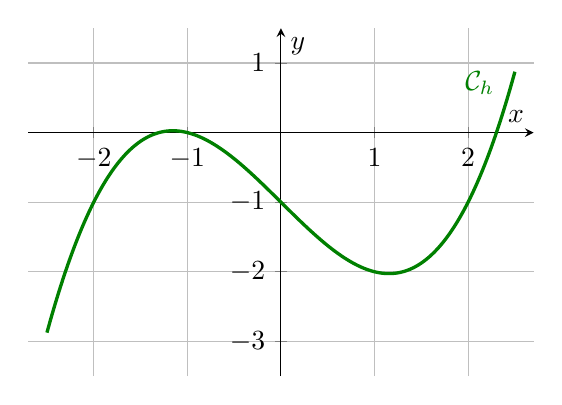
\begin{tikzpicture}
\begin{axis}[
    axis lines=middle,
    xmin=-2.7, xmax=2.7,
    ymin=-3.5, ymax=1.5,
    domain=-2.5:2.5,
    samples=300,
    grid=major,
    xtick={-2,-1,0,1,2},
    ytick={-3,-2,-1,0,1},
    xlabel={\(x\)},
    ylabel={\(y\)},
    width=8cm,
    height=6cm
]
\addplot[green!50!black, very thick] {1/3*(x+2)*x*(x-2)-1}
node[pos=0.95, above left] {\(\mathcal{C}_h\)};
\end{axis}
\end{tikzpicture}
\end{center}

\begin{enumerate}
    \item Quel est l'ensemble de définition de \(h\) ? \hfill /1
    \item Donner les images de \(-2\), \(-1\) et \(1\) par \(h\). \hfill /1
    \item Donner les éventuels antécédents de \(-1\) et de \(-2\). \hfill /1
\end{enumerate}

\columnbreak

\interroversion{D}

\textbf{Exercice 1 -- Tableau de valeurs \hfill /2}

On considère la fonction \(f\) définie sur \(\mathbb{R}\) par \(f(x)=x^2+2x-1\).

Complétez le tableau de valeurs suivant (une valeur est déjà calculée à titre d'exemple : \(f(0)=0^2+2\times 0-1=-1\)).

\begin{center}
    \renewcommand{\arraystretch}{1.5}
    \setlength{\tabcolsep}{0.25cm}
    \begin{tabular}{|*{7}{c|}}
    \hline
    \(x\) & \(-2\) & \(-1\) & \(0\) & \(1\) & \(2\) & \(3\) \\
    \hline
    \(f(x)\) & \(-1\) & & \(-1\) & \(2\) & & \(14\) \\
    \hline
    \end{tabular}
\end{center}

\vspace{3cm}

\textbf{Exercice 2 -- Lecture graphique \hfill /3}

On considère une fonction \(h\) dont la représentation graphique est donnée ci-dessous.

\begin{center}
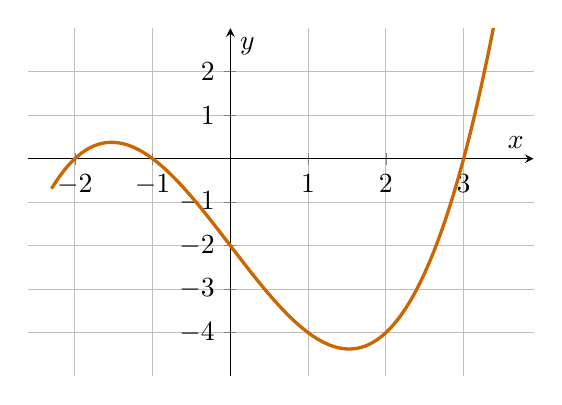
\begin{tikzpicture}
\begin{axis}[
    axis lines=middle,
    xmin=-2.6, xmax=3.9,
    ymin=-5, ymax=3,
    domain=-2.3:3.5,
    samples=300,
    grid=major,
    xtick={-2,-1,0,1,2,3},
    ytick={-4,-3,-2,-1,0,1,2},
    xlabel={\(x\)},
    ylabel={\(y\)},
    width=8cm,
    height=6cm
]
\addplot[orange!80!black, very thick] {1/3*(x+2)*(x+1)*(x-3)}
node[pos=0.95, above left] {\(\mathcal{C}_h\)};
\end{axis}
\end{tikzpicture}
\end{center}

\begin{enumerate}
    \item Quel est l'ensemble de définition de \(h\) ? \hfill /1
    \item Donner les images de \(-2\), \(0\) et \(2\) par \(h\). \hfill /1
    \item Donner les éventuels antécédents de \(0\) et de \(-4\). \hfill /1
\end{enumerate}

\end{sujets}

\end{document}
